%
% This is an example LaTeX file which uses the SANDreport class file.
% It shows how a SAND report should be formatted, what sections and
% elements it should contain, and how to use the SANDreport class.
% It uses the LaTeX article class, but not the strict option.
% ItINLreport uses .eps logos and files to show how pdflatex can be used
%
% Get the latest version of the class file and more at
%    http://www.cs.sandia.gov/~rolf/SANDreport
%
% This file and the SANDreport.cls file are based on information
% contained in "Guide to Preparing {SAND} Reports", Sand98-0730, edited
% by Tamara K. Locke, and the newer "Guide to Preparing SAND Reports and
% Other Communication Products", SAND2002-2068P.
% Please send corrections and suggestions for improvements to
% Rolf Riesen, Org. 9223, MS 1110, rolf@cs.sandia.gov
%
\documentclass[pdf,12pt]{INLreport}
% pslatex is really old (1994).  It attempts to merge the times and mathptm packages.
% My opinion is that it produces a really bad looking math font.  So why are we using it?
% If you just want to change the text font, you should just \usepackage{times}.
% \usepackage{pslatex}
\usepackage{times}
\usepackage[FIGBOTCAP,normal,bf,tight]{subfigure}
\usepackage{amsmath}
\usepackage{amssymb}
\usepackage{soul}
\usepackage{pifont}
\usepackage{enumerate}
\usepackage{listings}
\usepackage{fullpage}
\usepackage{xcolor}          % Using xcolor for more robust color specification
\usepackage{ifthen}          % For simple checking in newcommand blocks
\usepackage{textcomp}
\usepackage{mathtools}
\usepackage{relsize}
\usepackage{lscape}
\usepackage[toc,page]{appendix}
\usepackage{RAVEN}

\newtheorem{mydef}{Definition}
\newcommand{\norm}[1]{\lVert#1\rVert}
%\usepackage[table,xcdraw]{xcolor}
%\usepackage{authblk}         % For making the author list look prettier
%\renewcommand\Authsep{,~\,}

% Custom colors
\definecolor{deepblue}{rgb}{0,0,0.5}
\definecolor{deepred}{rgb}{0.6,0,0}
\definecolor{deepgreen}{rgb}{0,0.5,0}
\definecolor{forestgreen}{RGB}{34,139,34}
\definecolor{orangered}{RGB}{239,134,64}
\definecolor{darkblue}{rgb}{0.0,0.0,0.6}
\definecolor{gray}{rgb}{0.4,0.4,0.4}

\lstset {
  basicstyle=\ttfamily,
  frame=single
}


\setcounter{secnumdepth}{5}
\lstdefinestyle{XML} {
    language=XML,
    extendedchars=true,
    breaklines=true,
    breakatwhitespace=true,
%    emph={name,dim,interactive,overwrite},
    emphstyle=\color{red},
    basicstyle=\ttfamily,
%    columns=fullflexible,
    commentstyle=\color{gray}\upshape,
    morestring=[b]",
    morecomment=[s]{<?}{?>},
    morecomment=[s][\color{forestgreen}]{<!--}{-->},
    keywordstyle=\color{cyan},
    stringstyle=\ttfamily\color{black},
    tagstyle=\color{darkblue}\bf\ttfamily,
    morekeywords={name,type},
%    morekeywords={name,attribute,source,variables,version,type,release,x,z,y,xlabel,ylabel,how,text,param1,param2,color,label},
}
\lstset{language=python,upquote=true}

\usepackage{titlesec}
\newcommand{\sectionbreak}{\clearpage}
\setcounter{secnumdepth}{4}

%\titleformat{\paragraph}
%{\normalfont\normalsize\bfseries}{\theparagraph}{1em}{}
%\titlespacing*{\paragraph}
%{0pt}{3.25ex plus 1ex minus .2ex}{1.5ex plus .2ex}

%%%%%%%% Begin comands definition to input python code into document
\usepackage[utf8]{inputenc}

% Default fixed font does not support bold face
\DeclareFixedFont{\ttb}{T1}{txtt}{bx}{n}{9} % for bold
\DeclareFixedFont{\ttm}{T1}{txtt}{m}{n}{9}  % for normal

\usepackage{listings}

% Python style for highlighting
\newcommand\pythonstyle{\lstset{
language=Python,
basicstyle=\ttm,
otherkeywords={self, none, return},             % Add keywords here
keywordstyle=\ttb\color{deepblue},
emph={MyClass,__init__},          % Custom highlighting
emphstyle=\ttb\color{deepred},    % Custom highlighting style
stringstyle=\color{deepgreen},
frame=tb,                         % Any extra options here
showstringspaces=false            %
}}


% Python environment
\lstnewenvironment{python}[1][]
{
\pythonstyle
\lstset{#1}
}
{}

% Python for external files
\newcommand\pythonexternal[2][]{{
\pythonstyle
\lstinputlisting[#1]{#2}}}

\lstnewenvironment{xml}
{}
{}

% Python for inline
\newcommand\pythoninline[1]{{\pythonstyle\lstinline!#1!}}

% Named Colors for the comments below (Attempted to match git symbol colors)
\definecolor{RScolor}{HTML}{8EB361}  % Sonat (adjusted for clarity)
\definecolor{DPMcolor}{HTML}{E28B8D} % Dan
\definecolor{JCcolor}{HTML}{82A8D9}  % Josh (adjusted for clarity)
\definecolor{AAcolor}{HTML}{8D7F44}  % Andrea
\definecolor{CRcolor}{HTML}{AC39CE}  % Cristian
\definecolor{RKcolor}{HTML}{3ECC8D}  % Bob (adjusted for clarity)
\definecolor{DMcolor}{HTML}{276605}  % Diego (adjusted for clarity)
\definecolor{PTcolor}{HTML}{990000}  % Paul

\def\DRAFT{} % Uncomment this if you want to see the notes people have been adding
% Comment command for developers (Should only be used under active development)
\ifdefined\DRAFT
  \newcommand{\nameLabeler}[3]{\textcolor{#2}{[[#1: #3]]}}
\else
  \newcommand{\nameLabeler}[3]{}
\fi
\newcommand{\alfoa}[1] {\nameLabeler{Andrea}{AAcolor}{#1}}
\newcommand{\cristr}[1] {\nameLabeler{Cristian}{CRcolor}{#1}}
\newcommand{\mandd}[1] {\nameLabeler{Diego}{DMcolor}{#1}}
\newcommand{\maljdan}[1] {\nameLabeler{Dan}{DPMcolor}{#1}}
\newcommand{\cogljj}[1] {\nameLabeler{Josh}{JCcolor}{#1}}
\newcommand{\bobk}[1] {\nameLabeler{Bob}{RKcolor}{#1}}
\newcommand{\senrs}[1] {\nameLabeler{Sonat}{RScolor}{#1}}
\newcommand{\talbpaul}[1] {\nameLabeler{Paul}{PTcolor}{#1}}
% Commands for making the LaTeX a bit more uniform and cleaner
\newcommand{\TODO}[1]    {\textcolor{red}{\textit{(#1)}}}
\newcommand{\xmlAttrRequired}[1] {\textcolor{red}{\textbf{\texttt{#1}}}}
\newcommand{\xmlAttr}[1] {\textcolor{cyan}{\textbf{\texttt{#1}}}}
\newcommand{\xmlNodeRequired}[1] {\textcolor{deepblue}{\textbf{\texttt{<#1>}}}}
\newcommand{\xmlNode}[1] {\textcolor{darkblue}{\textbf{\texttt{<#1>}}}}
\newcommand{\xmlString}[1] {\textcolor{black}{\textbf{\texttt{'#1'}}}}
\newcommand{\xmlDesc}[1] {\textbf{\textit{#1}}} % Maybe a misnomer, but I am
                                                % using this to detail the data
                                                % type and necessity of an XML
                                                % node or attribute,
                                                % xmlDesc = XML description
\newcommand{\default}[1]{~\\*\textit{Default: #1}}
\newcommand{\nb} {\textcolor{deepgreen}{\textbf{~Note:}}~}


%%%%%%%% End comands definition to input python code into document

%\usepackage[dvips,light,first,bottomafter]{draftcopy}
%\draftcopyName{Sample, contains no OUO}{70}
%\draftcopyName{Draft}{300}

% The bm package provides \bm for bold math fonts.  Apparently
% \boldsymbol, which I used to always use, is now considered
% obsolete.  Also, \boldsymbol doesn't even seem to work with
% the fonts used in this particular document...
\usepackage{bm}


% Define tensors to be in bold math font.
\newcommand{\tensor}[1]{{\bm{#1}}}

% Override the formatting used by \vec.  Instead of a little arrow
% over the letter, this creates a bold character.
\renewcommand{\vec}{\bm}

% Define unit vector notation.  If you don't override the
% behavior of \vec, you probably want to use the second one.
\newcommand{\unit}[1]{\hat{\bm{#1}}}
% \newcommand{\unit}[1]{\hat{#1}}

% Use this to refer to a single component of a unit vector.
\newcommand{\scalarunit}[1]{\hat{#1}}

% Aliases
\newcommand{\raven}{\texttt{RAVEN}}
\newcommand{\ravens}{\texttt{RAVEN}'s}
\newcommand{\plugin}{\raven{} Plugin}
\newcommand{\plugins}{\raven{} Plugins}


% \toprule, \midrule, \bottomrule for tables
\usepackage{booktabs}

% \llbracket, \rrbracket
\usepackage{stmaryrd}

\usepackage{hyperref}
\hypersetup{
    colorlinks,
    citecolor=black,
    filecolor=black,
    linkcolor=black,
    urlcolor=black
}

% Compress lists of citations like [33,34,35,36,37] to [33-37]
\usepackage{cite}

% If you want to relax some of the SAND98-0730 requirements, use the "relax"
% option. It adds spaces and boldface in the table of contents, and does not
% force the page layout sizes.
% e.g. \documentclass[relax,12pt]{SANDreport}
%
% You can also use the "strict" option, which applies even more of the
% SAND98-0730 guidelines. It gets rid of section numbers which are often
% useful; e.g. \documentclass[strict]{SANDreport}

% The INLreport class uses \flushbottom formatting by default (since
% it's intended to be two-sided document).  \flushbottom causes
% additional space to be inserted both before and after paragraphs so
% that no matter how much text is actually available, it fills up the
% page from top to bottom.  My feeling is that \raggedbottom looks much
% better, primarily because most people will view the report
% electronically and not in a two-sided printed format where some argue
% \raggedbottom looks worse.  If we really want to have the original
% behavior, we can comment out this line...
\raggedbottom
\setcounter{secnumdepth}{5} % show 5 levels of subsection
\setcounter{tocdepth}{5} % include 5 levels of subsection in table of contents

% ---------------------------------------------------------------------------- %
%
% Set the title, author, and date
%
\title{RAVEN Plugins Manual}
%\author{%
%\begin{tabular}{c} Author 1 \\ University1 \\ Mail1 \\ \\
%Author 3 \\ University3 \\ Mail3 \end{tabular} \and
%\begin{tabular}{c} Author 2 \\ University2 \\ Mail2 \\ \\
%Author 4 \\ University4 \\ Mail4\\
%\end{tabular} }


\author{ TODO authors
%\\Paul W. Talbot
%\\Andrea Alfonsi
%\\Cristian Rabiti
%\\Diego Mandelli
%\\Joshua Cogliati
%\\Congjian Wang
%\\Daniel P. Maljovec
%\\Curtis Smith
}
% \\James B. Tompkins}   Just people who actually ``developed'' a significant capability in the code should be placed here. Andrea
%\author{\textbf{\textit{Main Developers:}}  \\Andrea Alfonsi}
%\affil{Idaho National Laboratory, Idaho Falls, ID 83402}
%\\\{cristian.rabiti, andrea.alfonsi, joshua.cogliati, diego.mandelli, robert.kinoshita, ramazan.sen\}@inl.gov}

% There is a "Printed" date on the title page of a SAND report, so
% the generic \date should [WorkingDir:]generally be empty.
\date{}


% ---------------------------------------------------------------------------- %
% Set some things we need for SAND reports. These are mandatory
%
\SANDnum{INL/EXT-TODO}
\SANDprintDate{\today}
\SANDauthor{TODO authors} %Andrea Alfonsi, Cristian Rabiti, Diego Mandelli, Joshua Cogliati, Congjian Wang, Paul W. Talbot, Daniel P. Maljovec, Curtis Smith}
\SANDreleaseType{Revision 0}


% ---------------------------------------------------------------------------- %
% Include the markings required for your SAND report. The default is "Unlimited
% Release". You may have to edit the file included here, or create your own
% (see the examples provided).
%
% \include{MarkOUO} % Not needed for unlimted release reports

\def\component#1{\texttt{#1}}

% ---------------------------------------------------------------------------- %
\newcommand{\systemtau}{\tensor{\tau}_{\!\text{SUPG}}}

% Added by Sonat
\usepackage{placeins}
\usepackage{array}

\newcolumntype{L}[1]{>{\raggedright\let\newline\\\arraybackslash\hspace{0pt}}m{#1}}
\newcolumntype{C}[1]{>{\centering\let\newline\\\arraybackslash\hspace{0pt}}m{#1}}
\newcolumntype{R}[1]{>{\raggedleft\let\newline\\\arraybackslash\hspace{0pt}}m{#1}}

% end added by Sonat
% ---------------------------------------------------------------------------- %
%
% Start the document
%

\begin{document}

    \maketitle

    % ------------------------------------------------------------------------ %
    % An Abstract is required for SAND reports
    %
%    \begin{abstract}
%    \input abstract
%    \end{abstract}


    % ------------------------------------------------------------------------ %
    % An Acknowledgement section is optional but important, if someone made
    % contributions or helped beyond the normal part of a work assignment.
    % Use \section* since we don't want it in the table of context
    %
%    \clearpage
%    \section*{Acknowledgment}



%	The format of this report is based on information found
%	in~\cite{Sand98-0730}.


    % ------------------------------------------------------------------------ %
    % The table of contents and list of figures and tables
    % Comment out \listoffigures and \listoftables if there are no
    % figures or tables. Make sure this starts on an odd numbered page
    %
    \cleardoublepage		% TOC needs to start on an odd page
    \tableofcontents
    %\listoffigures
    %\listoftables


    % ---------------------------------------------------------------------- %
    % An optional preface or Foreword
%    \clearpage
%    \section*{Preface}
%    \addcontentsline{toc}{section}{Preface}
%	Although muggles usually have only limited experience with
%	magic, and many even dispute its existence, it is worthwhile
%	to be open minded and explore the possibilities.


    % ---------------------------------------------------------------------- %
    % An optional executive summary
    %\clearpage
    %\section*{Summary}
    %\addcontentsline{toc}{section}{Summary}
    %\input{Summary.tex}
%	Once a certain level of mistrust and skepticism has
%	been overcome, magic finds many uses in todays science



%	and engineering. In this report we explain some of the
%	fundamental spells and instruments of magic and wizardry. We
%	then conclude with a few examples on how they can be used
%	in daily activities at national Laboratories.


    % ---------------------------------------------------------------------- %
    % An optional glossary. We don't want it to be numbered
%    \clearpage
%    \section*{Nomenclature}
%    \addcontentsline{toc}{section}{Nomenclature}
%    \begin{description}
%          \item[alohomoral]
%           spell to open locked doors and containers
%          \item[leviosa]
%           spell to levitate objects
%    \item[remembrall]
%           device to alert you that you have forgotten something
%    \item[wand]
%           device to execute spells
%    \end{description}


    % ---------------------------------------------------------------------- %
    % This is where the body of the report begins; usually with an Introduction
    %
    \SANDmain		% Start the main part of the report





\input{introduction.tex}
\input{making_new_plugin.tex}

Entities in RAVEN that are ready for new strategies via Plugins are
described in the following sections.

\section{ExternalModel plugins}
\label{sec:newExternalModelPlugin}
\begin{figure}
\centering
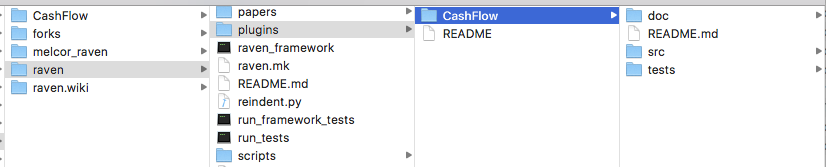
\includegraphics[width=1.0\textwidth]{pics/plugins_location.png}
\caption{Plugins Location}
\label{fig:pluginsLocation}
\end{figure}
The procedure of adding a plugin for the ExternalModel is a straightforward  process.
The addition of a plugin does not require modifying RAVEN itself.
Instead, the developer creates a new Python module that is going to be embedded
 in RAVEN at run-time (no need to introduce  hard-coded statements).
 This plugin needs to be placed in a folder (whatever name) located in (see figure~\ref{fig:pluginsLocation}):
\begin{lstlisting}[language=bash]
 path/to/raven/plugins/
\end{lstlisting}
In order to install a new plugin, the user can run the script contained in the RAVEN script folder:
\begin{lstlisting}[language=bash]
 python path/to/raven/scripts/install_plugins.py  **directory**
\end{lstlisting}
where  $**directory**$ should be replaced with the absolute path to the plugin directory.
(e.g. ``path/to/my/plugins/folder''). If the plugin developer wants to make of his plugin
an official supported plugin in RAVEN (by the submodule system), he needs to check
the raven wiki under the ``contribution'' section).

At the initialization stage, RAVEN imports all the Plugins that are contained in this directory and performs some preliminary cross-checks.
\\It is important to notice that the name of class in the Plugin module is the one the user needs to specify when the new plugin
needs to be used. For example, if the Plugin module contains the class 	``NewPlugin'', the \textit{subType} in the \xmlNode{ExternalModel} block will be 	``NewPlugin'':
\begin{lstlisting}[language=python]
  class NewPlugin(ExternalModelPluginBase):
    ...
\end{lstlisting}
\begin{lstlisting}[style=XML,morekeywords={name,file}] %moreemph={name,file}]
  <Models>
    ...
    <ExternalModel name='whatever' subType='NewPlugin'>
     ...
    </ExternalModel>
    ...
  </Models>
\end{lstlisting}

In the following sub-sections, a step-by-step procedure for creating a new ExternalModel plugin is outlined.

\subsection{ExternalModel Plugin Input}
\label{subsec:externalModelPluginInput}
When a new ExternalModel plugin is developed, its RAVEN input is almost identical
to the general ExternalModel entity (see \ref{subsec:models_externalModel}).
The specifications of an ExternalModel Plugin must be defined within the XML block
\xmlNode{ExternalModel}.
%
This XML node needs to contain the attributes:

\vspace{-5mm}
\begin{itemize}
  \itemsep0em
  \item \xmlAttr{name}, \xmlDesc{required string attribute}, user-defined name
  of this External Model.
  %
  \nb As with the other objects, this is the name that can be used to refer to
  this specific entity from other input blocks in the XML.
  \item \xmlAttr{subType}, \xmlDesc{required string attribute}, must be equal to the
  name of the new plugin the user wants to use (e.g. $NewPlugin$).
  \nb In case a plugin is requested (through the  \xmlAttr{subType} attribute) the
  attribute \xmlAttr{ModuleToLoad} must not be inputted.
  %
\end{itemize}
\vspace{-5mm}

In order to make the RAVEN code aware of the variables the user is going to
manipulate/use in her/his ExternalModel Plugin, the variables need to be specified
in the \xmlNode{ExternalModel} input block.
%
The user needs to input, within this block, only the variables that RAVEN needs
to be aware of (i.e. the variables are going to directly be used by the Plugin)
and not the local variables that the ExternalModel Plugin developer does not want to,
for example, store in a RAVEN internal object.
%
These variables are specified within a \xmlNode{variables} block:
\begin{itemize}
  \item \xmlNode{variables}, \xmlDesc{string, required parameter}.
  %
  Comma-separated list of variable names.
  %
  Each variable name needs to match a variable used/defined in the external python
  model.
  %
\end{itemize}

In addition, if the user wants to use the alias system, the following XML block can be used as
described in the RAVEN user manual under Models.

When the Plugin variables are defined, at run time, RAVEN initializes
them and tracks their values during the simulation.
%
Each variable defined in the \xmlNode{ExternalModel} block is available in the
Plugin class (in each implemented method ) as the object ``container'' that ``acts''
as a Python ``self''. For example,
\begin{lstlisting}[language=python]
  def run (self, container, inputs):
    print(container.variableA)
\end{lstlisting}

%%%%%%%
\subsection{ExternalModel Plugin Creation}
\label{subsec:externalModelPluginCreation}
As already mentioned, RAVEN imports all the ``ExternalModel Plugins'' at run-time.
In order to make RAVEN
able to drive a newer ExternalModel plugin, the developer needs to code a Python class
containing few methods (with strict syntax) that are called by RAVEN during the simulation.
\\ Every new ``ExternalModel Plugin'' must inherit from a RAVEN base class named
$ExternalModelPluginBase$:
\begin{lstlisting}[language=python]
  class NewPlugin(ExternalModelPluginBase):
    ...
\end{lstlisting}
This base class is needed by RAVEN to identify in the plugins folder which class must
be considered an  ``ExternalModel Plugin''.
\\ In addition, when loading an ``ExternalModel Plugin'', RAVEN expects to find, in the class representing the plugin,
 the following required methods:
\begin{lstlisting}[language=python]
from ExternalModelPluginBase import ExternalModelPluginBase
class NewPlugin(ExternalModelPluginBase):
  def run (self, container, Inputs)
\end{lstlisting}
In addition, the following optional methods can be specified:
\begin{lstlisting}[language=python]
from ExternalModelPluginBase import ExternalModelPluginBase
class NewPlugin(ExternalModelPluginBase):
  ...
  def createNewInput(self, container, inputs, samplerType, **Kwargs)
  def _readMoreXML(self, container, xmlNode)
  def initialize(self,container, runInfo, inputs)
\end{lstlisting}
In the following sub-sections all the methods are fully explained, providing examples.
\subsubsection{Method: \texttt{run}}
\label{subsubsec:runExternalModelPlugin}
\begin{lstlisting}[language=python]
def run (self, container, Inputs)
\end{lstlisting}
As stated previously, the only method that \emph{must} be present in an
ExternalModel Plugin is the \textbf{run} function.
%
In this function, the plugin developer needs to implement the algorithm that RAVEN will
execute.
%
The \texttt{\textbf{run}} method is generally called after having inquired the
``createNewInput'' method (either the internal RAVEN one or the one implemented by
the plugin developer).
%
The only two attributes this method is going to receive are a Python list of inputs
(the inputs coming from the \texttt{createNewInput} method) and a ``self-like'' object
named ``container''.
%
If the user wants RAVEN to collect the results of this method, the outcomes of
interest need to be stored in the above mentioned ``container'' object.
%
\nb RAVEN is trying to collect the values of the variables listed only in the
\xmlNode{ExternalModel} XML block.
%
In the following an example is reported:
\begin{lstlisting}[language=python]
def run(self, container, Input):
  # in here the actual run of the
  # model is implemented
  input = Input[0]
  container.outcome = container.sigma*container.rho*input[``whatEver'']
\end{lstlisting}

\subsubsection{Method: \texttt{createNewInput}}
\label{subsubsec:createNewInputExternalModelPlugin}
\begin{lstlisting}[language=python]
def createNewInput(self, container, inputs, samplerType, **Kwargs)
\end{lstlisting}

The \textbf{createNewInput} method can be implemented by the ExternalModel Plugin
developer to create a new input with the information coming from the RAVEN framework.
%
In this function, the developer can retrieve the information coming from the RAVEN
framework, during the employment of a calculation flow, and use them to
construct a new input that is going to be transferred to the ``run'' method.
%
The new input created needs to be returned to RAVEN (i.e. ``return NewInput'').
\\This method expects that the new input is returned in a Python ``dictionary''.
%
RAVEN communicates, thorough a set of method attributes, all the information
that are generally needed to create a new input:

\begin{itemize}
  \item \texttt{inputs}, \xmlDesc{python list}, a list of all the inputs that
  have been defined in the ``Step'' using this model.
  \item \texttt{samplerType}, \xmlDesc{string}, the type of Sampler, if a
  sampling strategy is employed; will be None otherwise.
  \item \texttt{Kwargs}, \xmlDesc{dictionary}, a dictionary containing several
  pieces of information (that can change based on the ``Step'' type).
  %
  If a sampling strategy is employed, this dictionary contains another
  dictionary identified by the keyword ``SampledVars'', in which the variables
  perturbed by the sampler are reported.
\end{itemize}
\nb If the ``Step'' that is using this Model has as input(s) an object of main
class type ``DataObjects'' (see Section~\ref{sec:DataObjects}), the internal ``createNewInput''
method is going to convert it in a dictionary of values.
%
Here we present an example:
\begin{lstlisting}[language=python]
def createNewInput(self, container, inputs,samplerType,**Kwargs):
  # in here the actual createNewInput of the
  # model is implemented
  if samplerType == 'MonteCarlo':
    avariable = inputs['something']*inputs['something2']
  else:
    avariable = inputs['something']/inputs['something2']
  return avariable*Kwargs['SampledVars']['aSampledVar']
\end{lstlisting}

\subsubsection{Method: \texttt{\_readMoreXML}}
\label{subsubsec:externalReadMoreXMLExternalModelPlugin}
\begin{lstlisting}[language=python]
def _readMoreXML(self, container, xmlNode)
\end{lstlisting}
As already mentioned, the \textbf{\_readMoreXML} method can be implemented by the
ExternalModel Plugin developer if the XML input that belongs to this ExternalModel
plugin needs to be extended to contain other information.
%
The read information needs to be stored in the ``self-like'' object ``container''
 in order to be available to all the other methods (e.g. if the developer needs to add a
 couple of newer XML nodes with information needed by the algorithm implemented in
 the ``run'' method).
%
If this method is implemented in the \textbf{ExternalModel}, RAVEN is going to
call it when the node \xmlNode{ExternalModel} is found parsing the XML input
file.
%
The method receives from RAVEN an attribute of type ``xml.etree.ElementTree'',
containing all the sub-nodes and attribute of the XML block \xmlNode{ExternalModel}.
%

Example XML:
\begin{lstlisting}[style=XML,morekeywords={subType,ModuleToLoad}]
<Simulation>
  ...
  <Models>
     ...
    <ExternalModel name='AnExtModule' subType=''NewPlugin">
       <variables>sigma,rho,outcome</variables>
       <!--
          here we define other XML nodes RAVEN does not read automatically.
          We need to implement, in the external model Plugin class the _readMoreXML
          method
        -->
        <newNodeWeNeedToRead>
         whatNeedsToBeRead
        </newNodeWeNeedToRead>
    </ExternalModel>
     ...
  </Models>
  ...
</Simulation>
\end{lstlisting}

Corresponding Python function:
\begin{lstlisting}[language=python]
def _readMoreXML(self, container, xmlNode):
  # the xmlNode is passed in by RAVEN framework
  # <newNodeWeNeedToRead> is unknown (in the RAVEN framework)
  # we have to read it on our own
  # get the node
  ourNode = xmlNode.find('newNodeWeNeedToRead')
  # get the information in the node
  container.ourNewVariable = ourNode.text
  # end function
\end{lstlisting}

\subsubsection{Method: \texttt{initialize}}
\label{subsubsec:externalInitializeExternalModelPlugin}
\begin{lstlisting}[language=python]
def initialize(self, container, runInfo, inputs)
\end{lstlisting}

The \textbf{initialize} method can be implemented in the \textbf{ExternalModel} Plugin
in order to initialize some variables needed by it.
%
For example, it can be used to compute a quantity needed by the ``run'' method
before performing the actual calculation.
%
If this method is implemented in the \textbf{ExternalModel} Plugin, RAVEN is going to
call it at the initialization stage of each ``Step'' (see section \ref{sec:steps}).
%
RAVEN will communicate, thorough a set of method attributes, all the information
that are generally needed to perform an initialization:
\begin{itemize}
  \item runInfo, a dictionary containing information regarding how the
  calculation is set up (e.g. number of processors, etc.).
  %
  It contains the following attributes:
  \begin{itemize}
    \item \texttt{DefaultInputFile} -- default input file to use
    \item \texttt{SimulationFiles} -- the xml input file
    \item \texttt{ScriptDir} -- the location of the pbs script interfaces
    \item \texttt{FrameworkDir} -- the directory where the framework is located
    \item \texttt{WorkingDir} -- the directory where the framework should be
    running
    \item \texttt{TempWorkingDir} -- the temporary directory where a simulation
    step is run
    \item \texttt{NumMPI} -- the number of mpi process by run
    \item \texttt{NumThreads} -- number of threads by run
    \item \texttt{numProcByRun} -- total number of core used by one run (number
    of threads by number of mpi)
    \item \texttt{batchSize} -- number of contemporaneous runs
    \item \texttt{ParallelCommand} -- the command that should be used to submit
    jobs in parallel (mpi)
    \item \texttt{numNode} -- number of nodes
    \item \texttt{procByNode} -- number of processors by node
    \item \texttt{totalNumCoresUsed} -- total number of cores used by driver
    \item \texttt{queueingSoftware} -- queueing software name
    \item \texttt{stepName} -- the name of the step currently running
    \item \texttt{precommand} -- added to the front of the command that is run
    \item \texttt{postcommand} -- added after the command that is run
    \item \texttt{delSucLogFiles} -- if a simulation (code run) has not failed,
    delete the relative log file (if True)
    \item \texttt{deleteOutExtension} -- if a simulation (code run) has not
    failed, delete the relative output files with the listed extension (comma
    separated list, for example: `e,r,txt')
    \item \texttt{mode} -- running mode, curently the only mode supported is
      mpi (but custom modes can be created)
    \item \textit{expectedTime} -- how long the complete input is expected to
    run
    \item \textit{logfileBuffer} -- logfile buffer size in bytes
  \end{itemize}
  \item inputs, a list of all the inputs that have been specified in the
  ``Step'' using this model.
  %
\end{itemize}
As all the others method in the ExternalModel Plugin, the information \emph{must} be
stored in the ``self-like'' object ``container''.
In the following an example is reported:
\begin{lstlisting}[language=python]
def initialize(self, container, runInfo, inputs):
 # Let's suppose we just need to initialize some variables
  container.sigma = 10.0
  container.rho   = 28.0
  # end function
\end{lstlisting}


\section{Plots}
\label{sec:outstreams_plot}
New plots that are specific to particular applications are possible through \xmlNode{OutStreams}
\xmlNode{Plot} plugins.

These plotting plugins should inherit from the \texttt{PlotPlugin} base class defined in
\begin{lstlisting}[language=bash]
  raven/framework/PluginBaseClasses/OutStreamPlotPlugin.py
\end{lstlisting}
which sets up the plotting tool to be found when RAVEN runs.

A good example of the \texttt{PlotPlugin} can be found in the RAVEN ExamplePlugin, found at
\begin{lstlisting}[language=bash]
  raven/plugins/ExamplePlugin/src/CorrelationPlot.py
\end{lstlisting}

There are a few methods that can or must be implemented for new plotting strategies.

%
%
\subsection{\texttt{run} method, required}
The \texttt{run} method is the primary execution method for the PlotPlugin. Here, whatever data
handling and plotting mechanics will be executed. Note that \texttt{run} does not receive any inputs;
often, the source for the data to be plotted will be identified in the \texttt{initialize} method.

The \texttt{run} method can perform many actions including data manipulation, creation of
\texttt{matplotlib} figures and axes, saving figures to file, and so forth. In the end, \texttt{run}
should not return anything.

%
%
\subsection{Constructor, optional}
As the constructor for Python classes, the \texttt{\_\_init\_\_} method should be extended to define
any instance variables used in the plugin class. If no instance variables are used, this may be ommitted.

Any call to \texttt{\_\_init\_\_} must include a call to the parent's constructor, such as
\begin{lstlisting}[language=python]
  def __init__(self):
    """ ... """
    super().__init__()
\end{lstlisting}
This assures access to basic RAVEN functionalities required to use the plugin.

%
%
\subsection{Input Handling methods, optional}
The class method \texttt{getInputSpecification} and corresponding instance method
\texttt{handleInput} are how RAVEN determines what user inputs are allowed and how those input
values get stored in the plugin. Acceptable inputs are defined in \texttt{getInputSpecification}
and then read in during \texttt{handleInput}. Both of these methods require a call to \texttt{super}
to function as expected.

%
%
\subsection{Initialization, optional}
The aptly-named \texttt{initialize} method is used at the start of every RAVEN \xmlNode{Step} to prepare
for execution. A common task for this method is to find the source of the data to plot. To make this
process easier, RAVEN provides a \texttt{self.findSource} method that can search the input dictionary
provided to \texttt{initialize} and find a \xmlNode{DataObject} by string name.

%
%





\clearpage
\begin{appendices}
  \section{Document Version Information}
  \input{../version.tex}
\end{appendices}
%\input{examplesPrimer.tex}


    % ---------------------------------------------------------------------- %
    % References
    %
    \clearpage
    % If hyperref is included, then \phantomsection is already defined.
    % If not, we need to define it.
    \providecommand*{\phantomsection}{}
    \phantomsection
    \addcontentsline{toc}{section}{References}
    \bibliographystyle{ieeetr}
    \bibliography{raven_plugins_manual}


    % ---------------------------------------------------------------------- %
    %

    % \printindex

    %\include{distribution}

\end{document}
